\subsection{Contour Detection}
\label{sec:contour-detection}

\subsubsection{Apply contour detection to the same dataset}
A contour follows a region's boundary. The baseline, all parameter experiments,
and the matched blob comparison cover all 1,310 images. The ten fixed display
examples are used only for illustrations, with identical prepared inputs for
both methods.

The grayscale image $I$ is smoothed by Gaussian filter $G_\sigma$, whose
standard deviation $\sigma$ controls smoothing strength. Brightness threshold
$t$ separates pixels into a binary mask $M$:
\begin{equation}
 M(x,y)=\begin{cases}1,&(G_\sigma*I)(x,y)>t,\\0,&\text{otherwise}.\end{cases}
 \label{eq:contour-mask}
\end{equation}
Here $(x,y)$ is pixel position and $*$ denotes convolution. This separation
is called \emph{segmentation}; the baseline uses $\sigma=1$ pixel and $t=0.5$.

ContourPy's marching-squares algorithm traces boundaries between mask values
0 and 1 at level 0.5. This fixed tracing level differs from the adjustable
image threshold $t$. Only closed curves (loops) of area at least
$A_{\min}=25$ square pixels are retained. Open curves are excluded;
outer boundaries and boundaries around holes count separately.

\subsubsection{Visualize contours using different colors}
Figure~\ref{fig:contour-example} overlays both methods on the same sedan.
Each contour has a distinct color, independent of vehicle class. Dashed boxes
mark the same rear-window region to support a direct comparison; they are
visual guides rather than annotated object boundaries.

\begin{figure}[H]
 \centering
 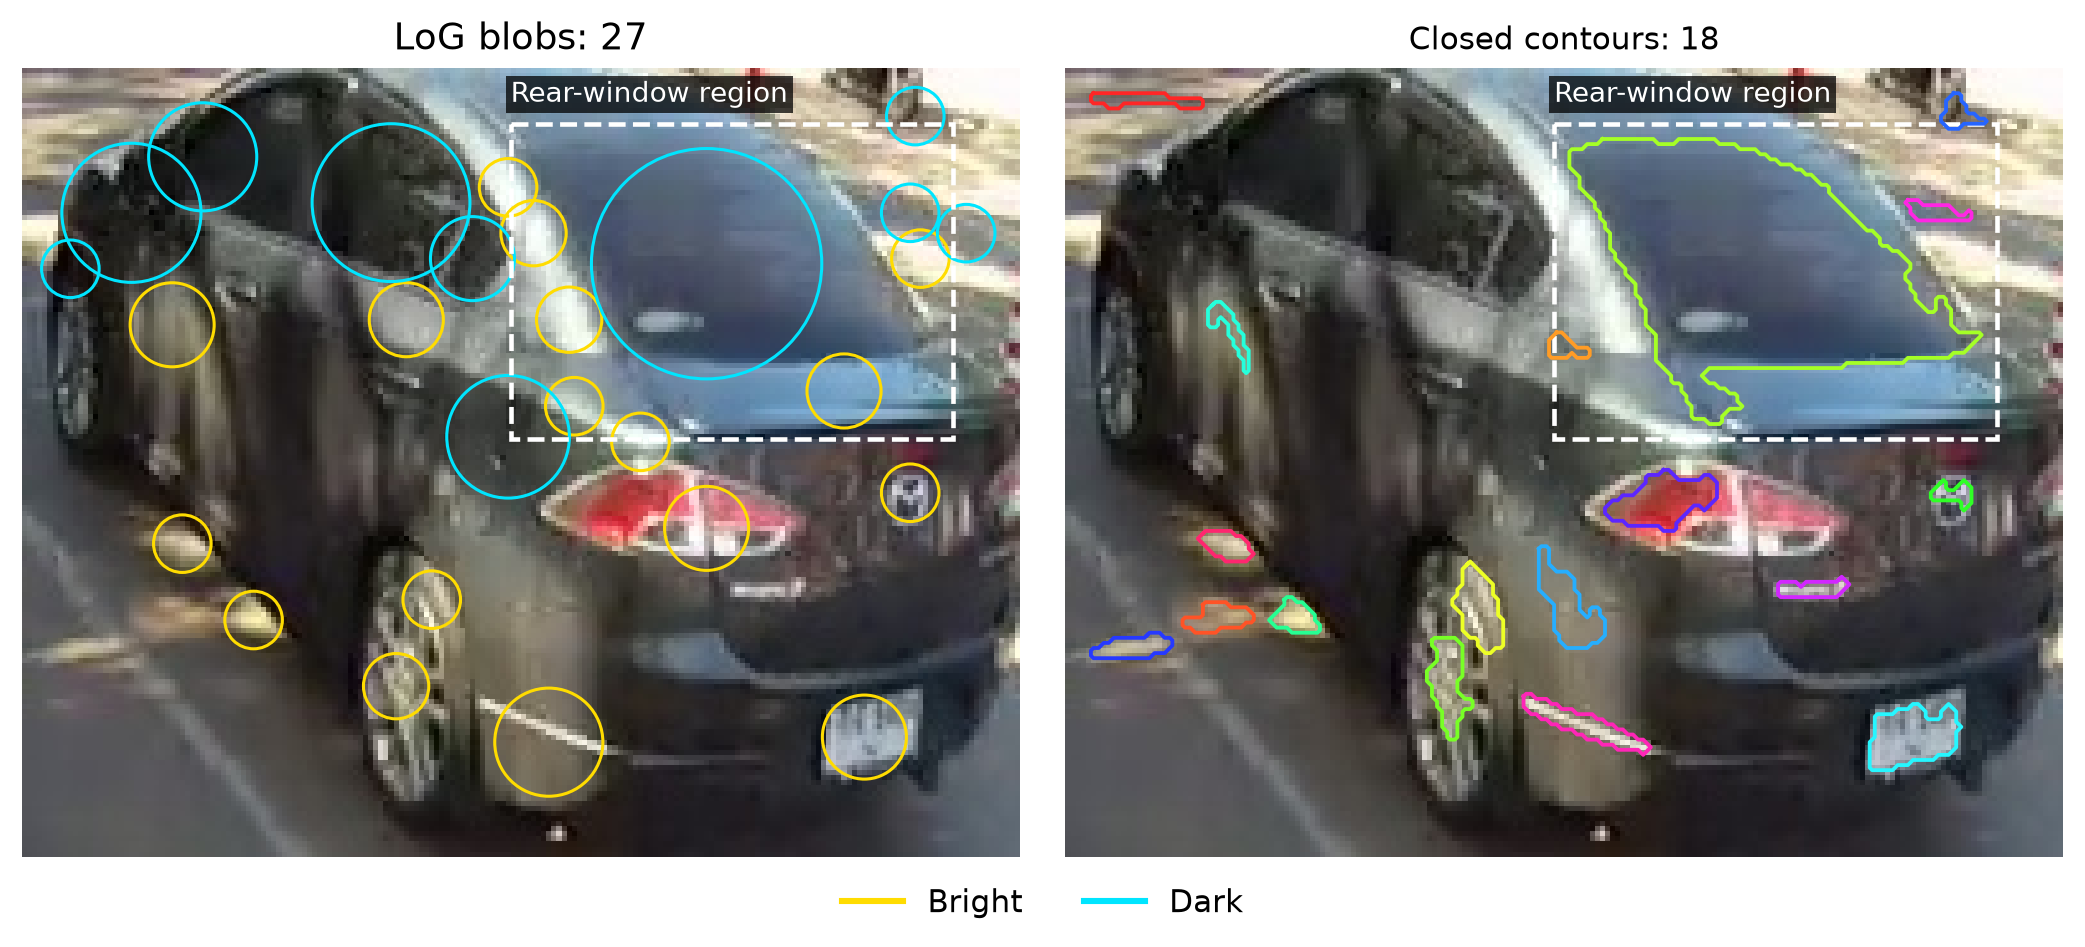
\includegraphics[width=\linewidth]{Images/blob_contour_window_comparison.png}
 \caption{Matched sedan example: 27 blobs (left) and 18 closed contours (right).
 Yellow/cyan circles mark bright/dark blobs; contour colors distinguish loops.
 Dashed boxes identify the same rear-window region.}
 \label{fig:contour-example}
\end{figure}

\subsubsection{Calculate counts, areas, and perimeters}
A loop's $n$ ordered boundary points $(x_i,y_i)$ form a polygon. Area $A$
is calculated from adjacent coordinates; perimeter $P$ sums segment lengths:
\begin{equation}
 A=\frac12\left|\sum_{i=1}^{n}(x_i y_{i+1}-x_{i+1}y_i)\right|,
 \qquad
 P=\sum_{i=1}^{n}\sqrt{(x_{i+1}-x_i)^2+(y_{i+1}-y_i)^2}.
 \label{eq:contour-geometry}
\end{equation}
The loop closes with $(x_{n+1},y_{n+1})=(x_1,y_1)$. Area uses square pixels
and perimeter pixels. The baseline retains 19,468 contours, with 0--63 per
image and median 14; three images have none. It excludes 21,604 open curves
and 44,907 undersized or invalid closed curves.
Table~\ref{tab:detection-image-stats} summarizes the full dataset by class;
CSV exports retain counts for every image and measurements for every contour.
Overlapping hole and outer-loop areas cannot be summed as net foreground area.

\begin{table}[H]
\centering
\small
\caption{Full-dataset contour baseline. Mean area $A$ (px$^2$) and perimeter
$P$ (px) are calculated over individual retained loops, including in the total row.}
\label{tab:detection-image-stats}
\begin{tabular}{lrrrr}
\toprule
Vehicle class & Images & Contours & Mean $A$ & Mean $P$ \\
\midrule
hatchback & 181 & 2,301 & 412.4 & 93.1 \\
motorcycle & 122 & 1,955 & 185.9 & 64.2 \\
pickup & 478 & 7,861 & 361.1 & 91.7 \\
sedan & 400 & 5,365 & 386.9 & 106.0 \\
suv & 129 & 1,986 & 381.6 & 103.6 \\
\midrule
Total & 1,310 & 19,468 & 358.8 & 94.3 \\
\bottomrule
\end{tabular}
\end{table}

\subsubsection{Compare blob and contour detection}
On the same 1,310 images, the baselines produce 85,074 blobs and 19,468 contours.
In the highlighted window of Figure~\ref{fig:contour-example}, a large cyan
circle summarizes the dark region by a center and radius. The green contour
follows its irregular mask boundary, extending below the glass where similar
intensities join. Smaller reflections produce additional local responses.
This shows the distinction between contrast scale and segmented shape:
neither representation guarantees the physical window boundary. Higher counts
do not indicate greater accuracy, and blob circle area and contour polygon
area are not interchangeable measurements.

\subsubsection{Discuss advantages and limitations}
LoG locates bright and dark features but cannot describe irregular outlines;
edges and reflections can produce repeated detections. Contours preserve
shape, but a single brightness threshold can merge unrelated regions or split
one object. Excluding open curves also removes frame-intersecting boundaries.
Full-dataset coverage quantifies these methods' behavior; annotated detections
would still be required to establish accuracy.

\subsubsection{Analyze threshold and filter-size effects}
Each experiment changes brightness threshold $t$, smoothing strength
$\sigma$, or minimum area $A_{\min}$ on all 1,310 images
(Table~\ref{tab:contour-parameters}). Figure~\ref{fig:contour-parameters}
shows the changes on one fixed pickup image.

\begin{table}[H]
\centering
\small
\caption{Contour parameter sensitivity across all 1,310 images. Means are
calculated over retained loops; area is in square pixels and perimeter in pixels.}
\label{tab:contour-parameters}
\begin{tabular}{llrrr}
\toprule
Setting & Value & Contours & Mean $A$ & Mean $P$ \\
\midrule
Baseline & Reference & 19,468 & 358.8 & 94.3 \\
Lower threshold & $t=0.35$ & 21,829 & 338.7 & 91.8 \\
Higher threshold & $t=0.65$ & 14,793 & 430.5 & 101.7 \\
No smoothing & $\sigma=0$ & 27,079 & 326.0 & 101.1 \\
Stronger smoothing & $\sigma=2$ & 12,066 & 450.9 & 91.9 \\
Larger minimum area & $A_{\min}=100$ & 8,639 & 745.1 & 161.3 \\
\bottomrule
\end{tabular}
\end{table}

\begin{figure}[H]
 \centering
 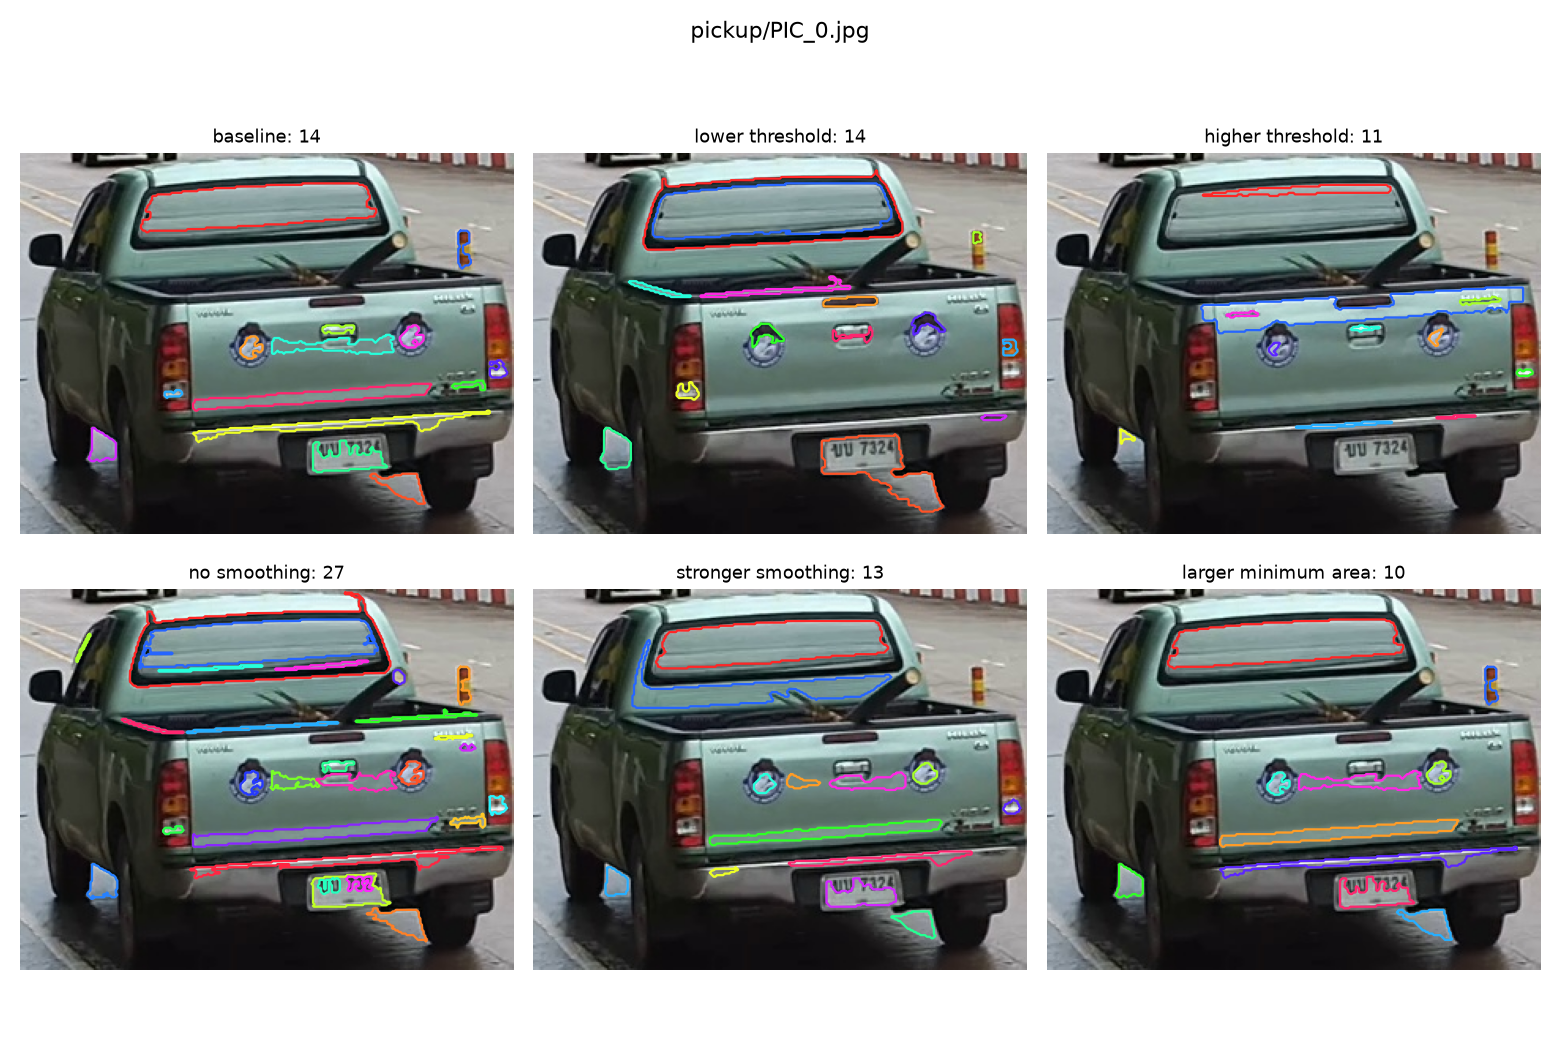
\includegraphics[width=0.92\linewidth]{Images/contour_parameters_pickup_PIC_0.png}
 \caption{Pickup contour experiments. Baseline and lower threshold both
 retain 14 loops despite different boundaries. Colors do not track loops
 between panels.}
 \label{fig:contour-parameters}
\end{figure}

\textbf{Threshold.} Raising $t$ reduces the total from 19,468 to 14,793,
but increases counts in 296 individual images. Changing pixel membership
can split or join regions, so the effect is not uniformly decreasing.
The pickup also illustrates why counts alone are insufficient: $t=0.35$ and
$t=0.5$ both retain 14 contours but produce different boundaries.

\textbf{Smoothing.} Without smoothing, fragmented detail raises the total
to 27,079; $\sigma=2$ reduces it to 12,066 and increases mean area from
358.8 to 450.9 square pixels. Fine regions disappear or merge, changing both
boundary geometry and the size distribution.

\textbf{Minimum area.} Raising $A_{\min}$ from 25 to 100 leaves 8,639
contours with mean area 745.1 square pixels. This removes existing small loops
without changing the mask or surviving boundaries. Parameter selection must
reflect the required detail and target region.

\subsubsection{Give examples of suitable applications}
LoG is suitable for locating candidate lamp details or reflective spots when
position and approximate scale are required. Contours support measurements
of irregular regions, such as the sedan window, if segmentation isolates the
boundary. Silhouette measurements require a contrasting background; shadows
and reflections limit this application in the present photographs.
\FloatBarrier
